\documentclass[14dd, a4paper]{article}

\usepackage{tikz}
\usetikzlibrary{shapes.geometric}

\begin{document}

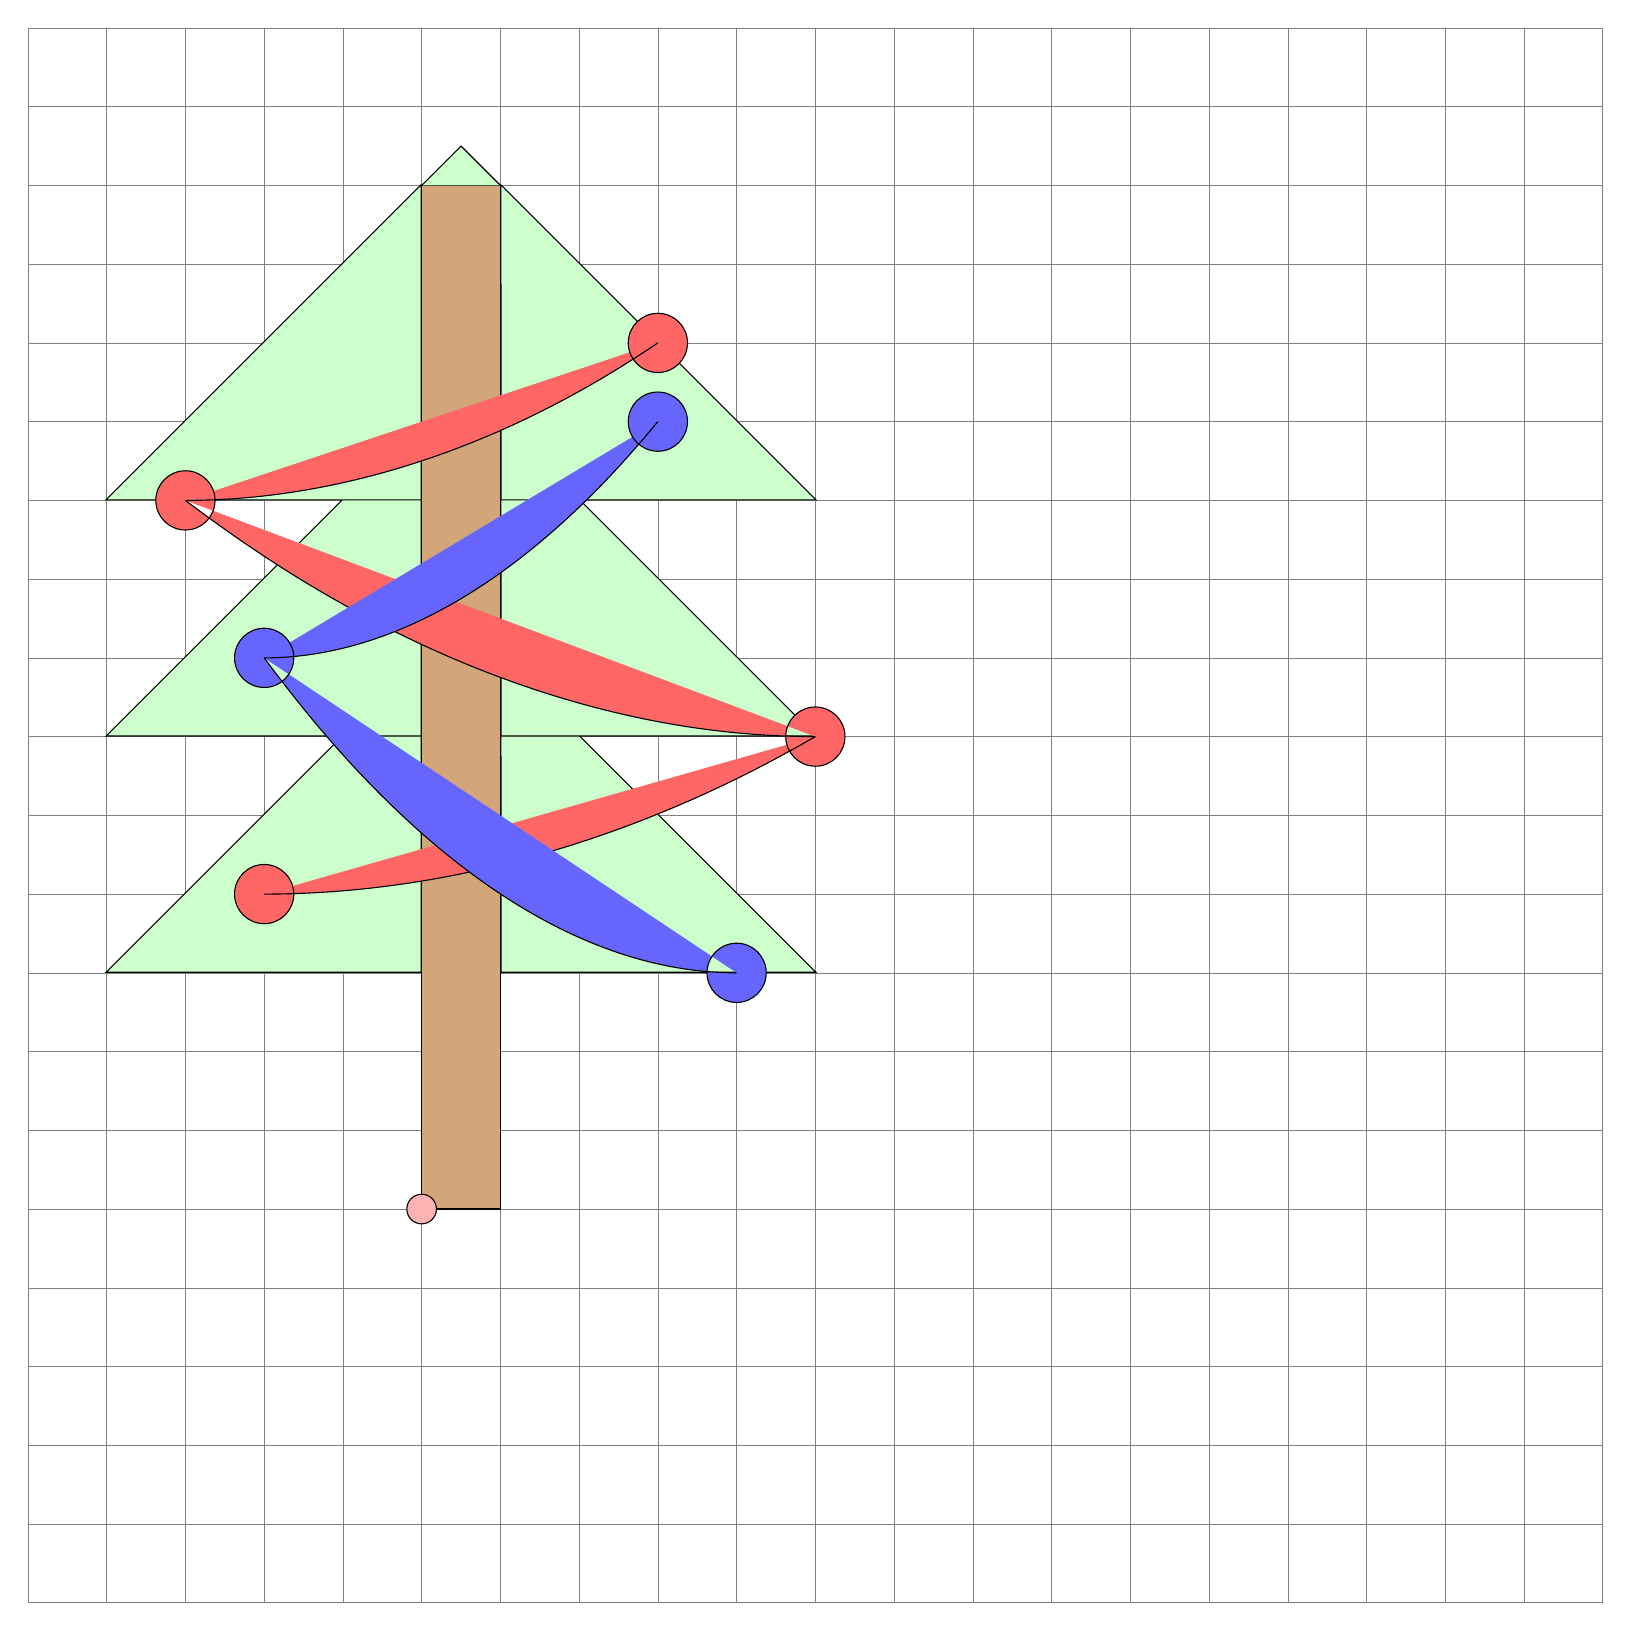
\begin{tikzpicture}[
trian R/.style = {isosceles triangle,
     isosceles triangle apex angle=90,
     minimum size=4cm/sqrt(2), inner sep=0pt,
     anchor=east,rotate=-135,
     draw, fill=green!20},
     trian L/.style = {isosceles triangle,
     rotate = 90,
     isosceles triangle apex angle=90,
     minimum size=4cm/sqrt(2), inner sep=0pt,
     anchor=east,rotate=-135,
     draw, fill=green!20}]

\draw[step=1cm,gray,very thin] (-5,-5) grid (15,15);
\draw[fill=brown!70] (0,0) rectangle (1,13);
\foreach \i in {1,...,3} {
      \node [trian R] at (1,3*\i){};  
    }
    \foreach \i in {1,...,3} {
      \node [trian L] at (0,3*\i){};  
    }
    \draw[fill=green!20] (0, 13) -- (0.5, 13.5) -- (1, 13);
    \draw[fill=red!30] (0,0) circle (5dd);
    \draw[fill=red!60] (-2,4) circle (10dd) -- (-2,4) parabola (5, 6) -- (5,6) circle (10dd) -- (5,6) parabola (-3, 9) -- (-3,9) circle (10dd) -- (-3,9) parabola (3, 11) -- (3,11) circle (10dd);
    \draw[fill=blue!60] (4,3) circle (10dd) -- (4,3) parabola (-2, 7) -- (-2, 7) circle (10dd) -- (-2,7) parabola (3, 10) -- (3,10) circle (10dd);

\end{tikzpicture}

\end{document}